\chapter{Daten und Zugrifsschichten}
\section{Einleitung}
Benutzer und App-Daten werden in zwei verschiedenen Datentöpfen gespeichert. Auf bestimmte Inhalte soll nur durch die Zugriffsschichten zugegriffen werden. Im Folgenden werden die Daten und die zugehörigen Zugrifsschichten aufgelistet.\\

\begin{figure}[htb]
    \centering
    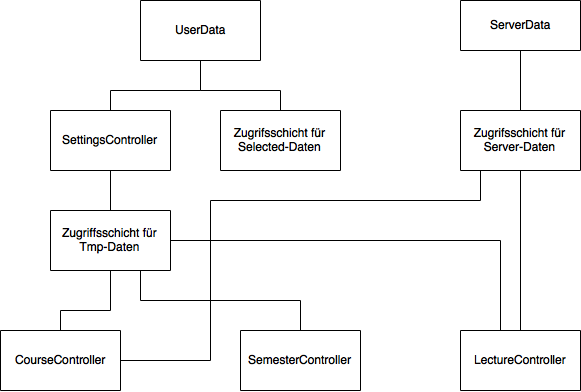
\includegraphics[width=\textwidth]{Daten}
    \caption{Daten und zugehörige Zugrifsschichten}
\end{figure}

Folgende Datentöpfe werden genutzt:
\begin{itemize}
     \item UserData
     \item ServerData \\
\end{itemize}

Folgende Zugrifssschichten sind vorhanden:
\begin{itemize}
     \item SelectedCourse
     \item SelectedSemester
     \item SelectedLectures
     \item AllChanges
     \item AllCourses
     \item AllLectures
\end{itemize}

\newpage
\section{UserData}
Alle Daten mit relevanten Informationen über den Nutzer werden in UserData gespeichert. Mit den Zugriffsschichten SelectedLectures, SelectedSemesters, SelectedCourses und AllChanges kann auf die Daten zugegriffen, die vom User gespeichert wurden. Diese Schichten haben nur einen lesenden Zugriff und können keine Daten manipulieren. \\

Für das Ändern der Daten ist die Tmp-Zugriffsschicht zuständig. Die Tmp Zugriffsschicht welche TmpSelectedLectures, TmpSelectedSemesters und TmpSelectedCourses beinhaltet, arbeitet mit einer eigenen Kopie von UserData. Dadurch können Veränderungen einfach wieder verworfen werden, da keine gespeicherten Daten veändern werden. Diese Zugriffsschichten werden nur im Einstellungen-Screen verwendet, um u. A. die ausgewählten Studeingänge, Semester und Vorlesungen festzuhalten. Erst beim Bestätigen der Eingaben werden die Daten aus der Kopie in das original UserData Übernommen. Die Kopie von UserData wird vom SettingsController verwaltet.\\

\begin{figure}[htb]
    \centering
    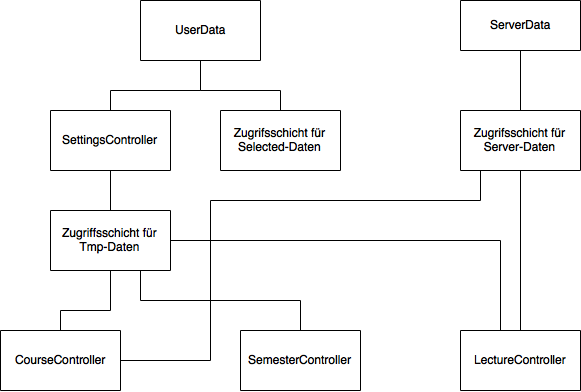
\includegraphics[width=\textwidth]{Daten}
    \caption{TO DO !!!}
\end{figure}

Im Folgenden wird der Inhalt von UserData und die zugeörigen Selekted und Tmp Zugrifsschichten beschrieben.\\

In UserData sind folgende Sachen enthalten:
\begin{itemize}
     \item gewählte Season (Sommer- oder Wintersemester)
     \item gewählte Studiengänge
     \item gewählte Semester
     \item gewählte Vorlesungen
     \item Stundenplanänderungen für gewählte Vorlesungen\\     
\end{itemize}

Selected-Zugrifsschichten: 
\begin{itemize}
     \item SelectedCourse: Ist für alle vom User selektierten Studiengänge zuständig
     \item SelectedSemester: Ist für alle vom User selektierten Semester zuständig
     \item SelectedLectures: Ist für alle vom User selektierten Vorlesungen zuständig
     \item AllChanges: Ist für Änderungen von gewählte Vorlesungen zuständig \\
\end{itemize}

Tmp-Zugrifsschichten: 
\begin{itemize}
     \item TmpCourse: Ist für alle vom User selektierten Studiengänge zuständig
     \item TmpSemester: Ist für alle vom User selektierten Semester zuständig
     \item TmpLectures: Ist für alle vom User selektierten Vorlesungen zuständig
     \item AllChanges: Ist für Änderungen von gewählte Vorlesungen zuständig 
\end{itemize}

\newpage
\section{ServerData}
Alle Daten die vom Server geladen wurden, werden in ServerData gespeichert. Durch die Zugriffsschichten AllLectures und AllCourses können die Daten abgefragt werden.

Folgenen wird über die in ServerData entahltenen Informationen und die zugehörigen Zugrifssschichten informiert.

In ServerData sind folgende Sachen enthalten:
\begin{itemize}
     \item Alle Studiengänge + Semester
     \item Alle Vorlesungen für ausgewählte Studiengänge + Semester \\     
\end{itemize}

Zugrifsschichten: 
\begin{itemize}
     \item AllCourses: Ist für alle geladenen Studiengänge + Semester zuständig
     \item AllLectures: Ist für alle geladenen Vorlesungen für Studiengänge + Semester zuständig\\
\end{itemize}

\newpage
\chapter{Hintergrundaktualisierung}
\section{Einleitung}
Die App soll im Hintergrund regelmäßig prüfen ob neue Stundenplanänderungen für den Benutzer entstanden sind.
Daher wurde der Background Fetch implementiert.
\begin{figure}[htb]
    \centering
    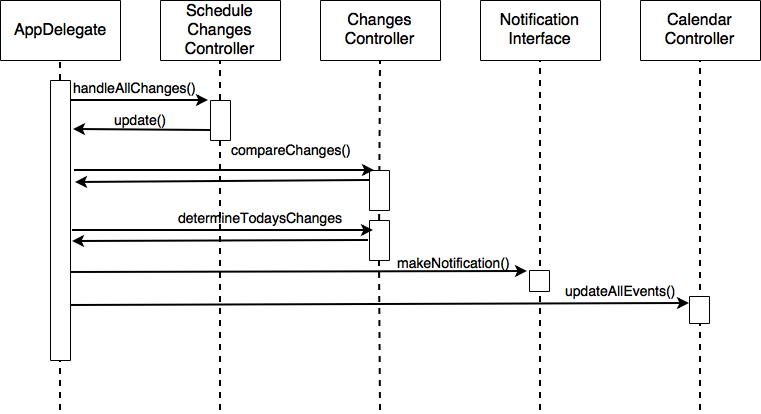
\includegraphics[width=\textwidth]{BackgroundFetch}
    \caption{Ablauf des Background Fetch}
\end{figure}

In diesem Sequenzdiagramm wird des Ablauf der application(performFetchWithCompletionHandler) Methode dargestellt. 
Zu Beginn werden durch den ScheduleChangesController die aktuellen Stundenplanänderungen vom Server geladen. 
Anschließend werden mit dem ChangesController die neu dazugekommenen Änderungen ermittelt und welche davon am aktuellen Tag stattfinden. Als Nächstes wird über das NotificationInterface eine lokale Notification für den User erstellt, die Ihn über die aktuellen Stundenplanänderungen informiert.
Zuletzt wird über den CalendarController der iOS Kalender aktualisiert.
